\documentclass[11pt,a4paper]{article}
\usepackage[utf8]{inputenc}
\usepackage[italian]{babel}
\usepackage{amsmath}
\usepackage{amsfonts}
\usepackage{amssymb}
\usepackage{graphicx}
\usepackage{caption}
\usepackage{subcaption}
\author{Volpini, Paganini, Finazzer, Beghini}
\title{Energia di Ionizzazione }
\begin{document}
\maketitle 
\section{Abstract}
Nella prima parte di questa esperienza si vuole studiare il fenomeno di produzione di correnti elettroniche per effetto termoionico in una camera da vuoto; in particolare si verificano sperimentalmente le leggi di Richardson e di Child. Nella seconda parte si studia invece il processo di ionizzazione di gas residui nella camera da vuoto; in particolare sperimentalmente si vogliono misurare le diverse energie di ionizzazione di alcune specie di gas.  
\section{Apparato sperimentale}



Come si evince dalla figura le principali componenti dell'apparato sperimentale sono:

\begin{figure}[!h]
  \begin{subfigure}[b]{0.6\textwidth}
    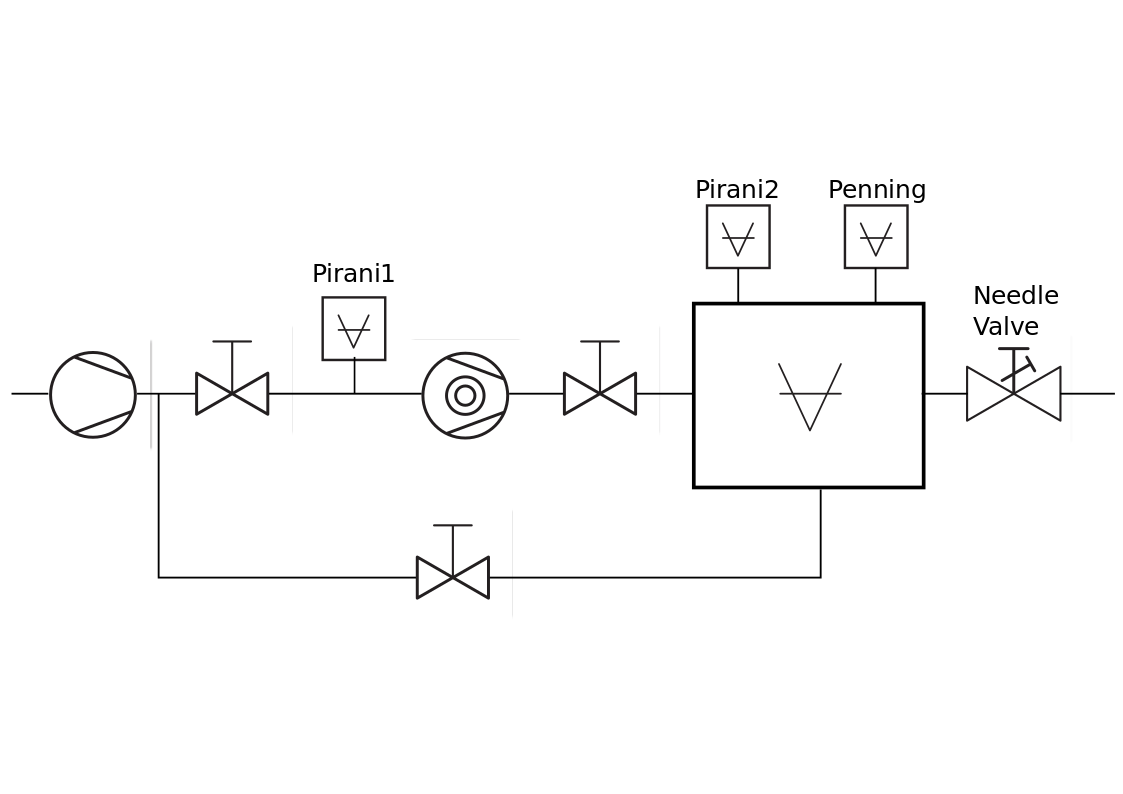
\includegraphics[width=\textwidth]{vuoto}
    \caption{schema apparato da vuoto} %eliminare intera riga se non si vuole didascalia
    \label{fig:f1}
  \end{subfigure}
  \hfill
  \begin{subfigure}[b]{0.4\textwidth}
    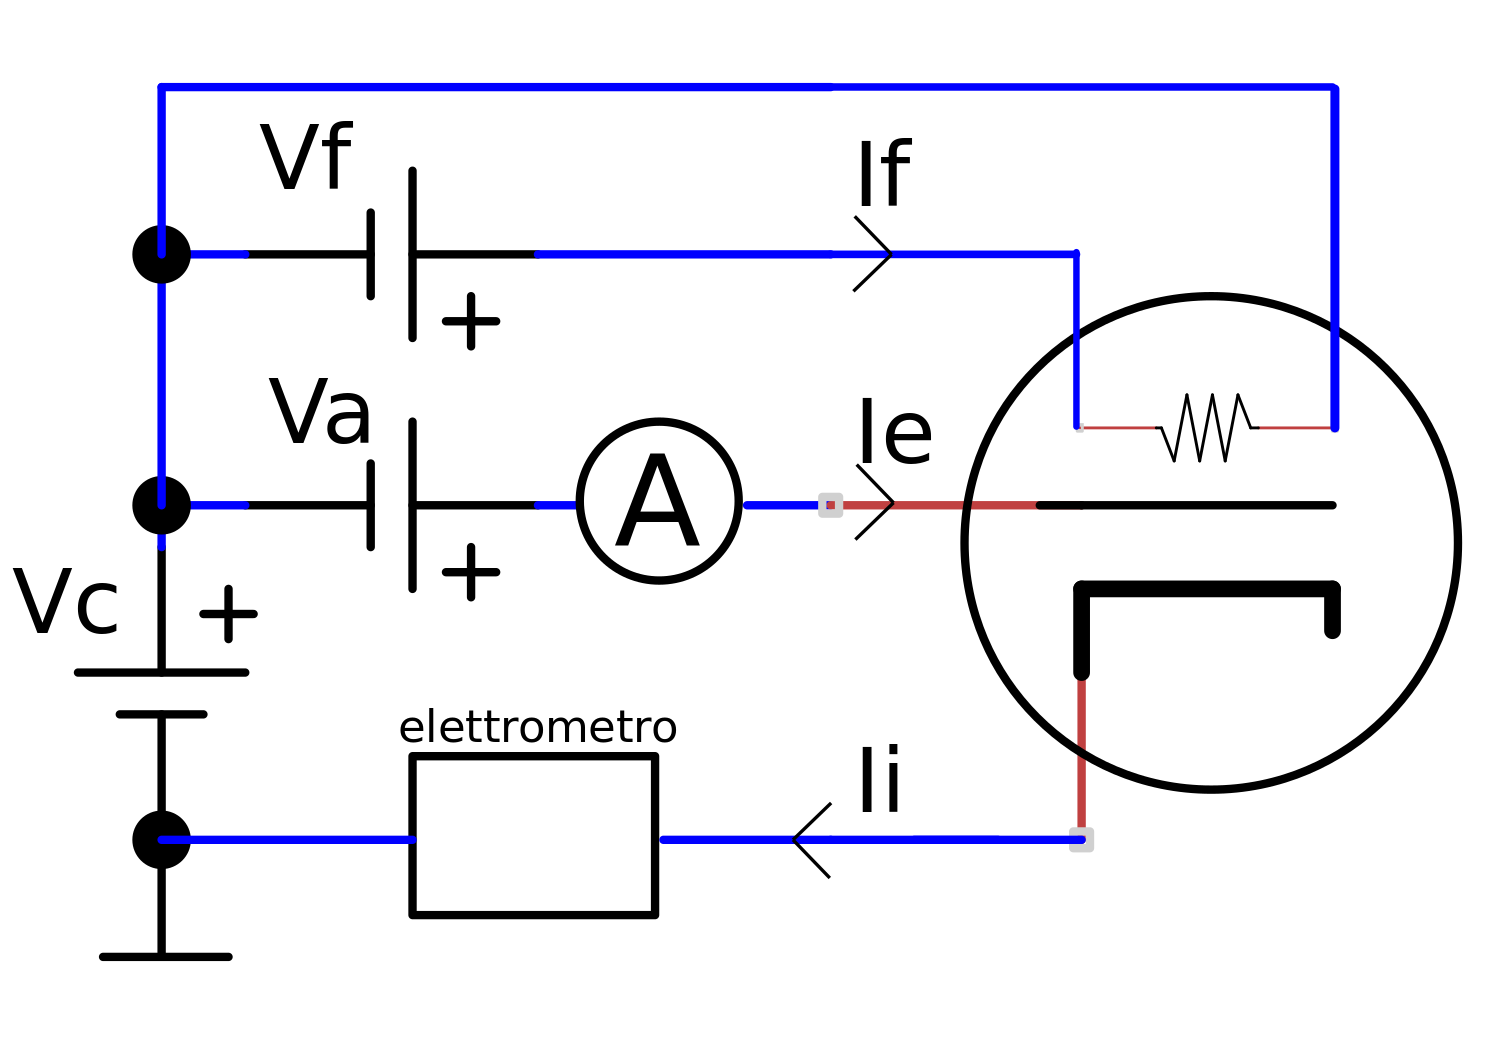
\includegraphics[width=\textwidth]{elettrico}
    \caption{schema circuito elettrico} %eliminare intera riga se non si vuole didascalia
    \label{fig:f2}
  \end{subfigure}
  %\caption{bla bla bla bla} %eliminare intera riga se non si vuole didascalia
\end{figure}

\begin{itemize}
\item camera da vuoto, 
\item misuratori di pressione Pennig (catodo freddo) e Pirani
\item pompa rotativa e pompa turbo-molecolare
\item valvola a spillo, valvola gate
\item flange di varie dimensioni
\item cavi banana-banana
\item valvola termoionica artigianale con filamento di tungsteno
\item generatori di corrente (Agilent e boh), multimetri digitali e palmari e un elettrometro
\end{itemize} 


\section{Prima parte}
Si comincia generando il vuoto all'interno della camera con le dovute accortezze. Si utilizzano pompa rotativa e pompa turbomolecolare per raggiungere condizioni di medio-alto vuoto ($P=10^{-6} mbar$).

Instauriamo una differenza di potenziale ai capi del filamento collegandone gli estremi rispettivamente uno a massa ed uno ad un generatore (per motivi sperimentali si è scelto quello in grado di erogare maggiori correnti); in questo modo è possibile riscaldare il filamento fino al raggiungimento di temperature tali da provocarne l'effetto termoionico (${T>1800 K}$). Il secondo generatore si usa invece per generare una differenza di potenziale tra filamento e anodo, e catturare quindi gli elettroni che si liberano dal filamento. Per la prima parte dell'esperienza il collettore rimane scollegato dal sistema in quanto non necessario.

\subsection{Dati sperimentali}

Si comincia con alcune misure specifiche del filamento del tungsteno utili a calcolare Resistenza e resistività dello stesso:
\begin{itemize}
\item diametro filamento ${d=205+-5\mu}$ 
\item lunghezza filamento ${l=20.70+-0.05mm}$
\item resistena (4 wire) filamento campione + fili ${}$
\item lunghezza filamento campione ${}$
\end{itemize}


Utilizziamo il filamento campione per calcolare la resistività del filamento utilizzato nella valvola termoionica (è una proprietà del materiale non del singolo filamento) $\rho=R_{s}\pi (d/2)^{2})/l_{s}=$ (qui dobbiamo utilizzare quelle citate sopra). Non utilizziamo il valore presentato nella letteratura scientifica in quanto la purezza del filamento in questione è sconosciuta (abbiamo comunque confrontato i due valori per quanto riguarda l'ordine di grandezza).

A questo punto è possibile calcolare la resistenza del filamento inserito nella valvola e soggetto ad effetto termoionico:
$ r_{fil}=l\rho/\pi (d/2)^{2})=$. 
dobbiamo a questo punto considerare il contributo alla resistenza dato dai cavi banana-banana utilizzati per il circuito in esame: calcoliamo la resistenza dei cavi mediante la relazione $r_{cavi}=r_{tot}-r_{fil}=$(modalità "4 wire" del multimetro). Supponendo che tali cavi non si riscaldino durante l'esperienza siamo in grado di separare i diversi contributi nel calcolo della resistenza $r_{tot}=r_{cavi}+r_{fil}$.

Successivamente si procede ad una stima della temperatura raggiunta dal filamento sottoposto ad una certa differenza di potenziale.
La letteratura scientifica fornisce la seguente relazione $\dfrac{r_{fil}}{r_{T300k}}=\alpha \Delta T $. Invertendo la relazione stimiamo la temperatura finale del filamento (dobbiamo mettere dei valori di temperatura: io metterei i due soglia).

Siamo ora interessati a verificare la legge di Richardon che studia l'andamento della corrente degli elettroni prodotti per effetto termoionico in funzione della temperatura del filamento (metterei la formula).
Impostiamo a questo punto alcuni parametri costanti (${P=2.7 \times 10^{-6} mbar}$, ${Va=50V}$, ) e procediamo a misurare valori di corrente elettronca al variare del potenziale di filamento ($V_{fil}$) e quindi della temperatura dello stesso (metterei i calcoli per passare da Vfil a Tfil).

\begin{figure}[h]
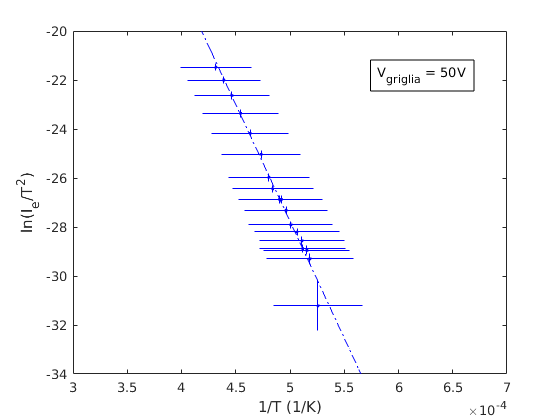
\includegraphics[width=\textwidth]{richardsonlin}
\end{figure}

Grafichiamo il logaritmo del rapporto tra corrente elettronica e quadrato della temperatura vs inverso della temperatura. Tramite regressione lineare calcoliamo la funzione lavoro: $W = (8.2 \pm 3.5) eV$. La letteratura fornisce la funzione lavoro di estrazione del tungsteno $\approx 4.32 \; - \; 5.22 \; eV$ compatibile solo nell'ordine di grandezza.  

	
Studiamo l'andamento della corrente elettronica in funzione del potenziale dell'anodo, concentrandoci nel range a bassi potenziali per verificare la legge di Child. In figura riportiamo i dati sperimentali con relativi fit. I parametri ottenuti da tali fit sono riportati in tabella.

\begin{center}
\begin{tabular}{|r|c|c|c|c|c|}
\hline

&\multicolumn{5}{|c|}{Temperature (K)}\\ \hline
&2406 $\pm$ 360& 	2318 $\pm$ 386&	2363 $\pm$ 393 &	2269 $\pm$ 377&	2238 $\pm$ 167\\ \hline
intercetta&	1.6&	0.7&	0.9&	0.4&	1.2\\ \hline
$[F C^{1/2} m^{-3/2}] \times 10^{-5}$&	$\pm$ 0.2&	$\pm$ 0.1&	$\pm$0.1&	$\pm$0.1&	$\pm$0.1	  \\ \hline
pendenza&	1.2 $\pm$ 0.1	&	1.6 $\pm$ 0.3&	1.5 $\pm$ 0.1&	1.6 $\pm$ 0.5&	1.5 $\pm$ 0.1\\ \hline 
\end{tabular}
\end{center}

I valori di pendenza corrispondono all'esponente del potenziale. La regressione lineare restituisce quindi valori confrontabili entro un sigma con il valore teorico 3/2. I valori delle temperature hanno un grosso errore che è dovuto principalmente dalla poca accuratezza nel misurare la lunghezza del filamento e la sua resistenza.

\begin{figure}[h]
%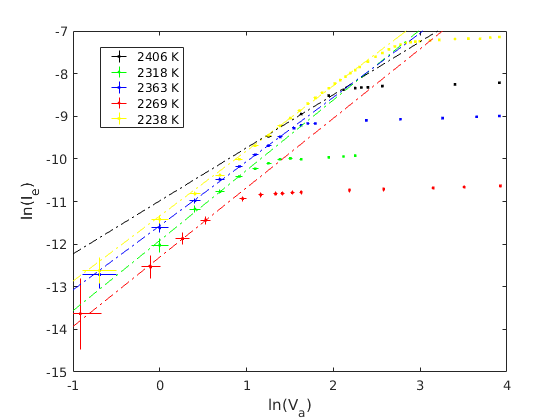
\includegraphics[scale=0.8]{child}
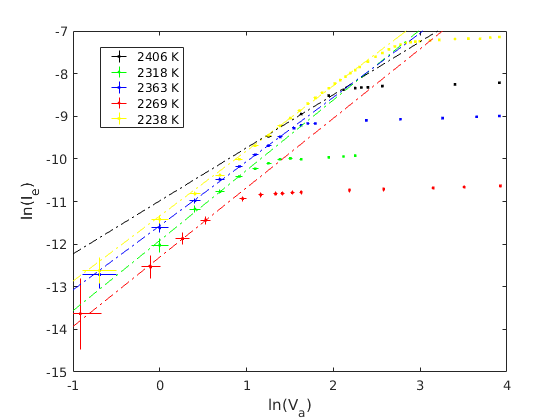
\includegraphics[width=\textwidth]{child}
\end{figure}

\newpage
\section{Seconda Parte}
 
Si procede in questa seconda parte dell'esperienza a studiare il fenomeno di ionizzazione di alcune specie di gas. Colleghiamo a questo punto opportunamente anche il collettore della valvola termoionica; in questo modo raccoglieremo gli atomi ionizzati sulla griglia esterna e ne potremmo misurare la corrente ionica. Accertandosi inoltre di tenere il collettore ad un potenziale inferiore rispetto al filamento si garantisce una barriera di potenziale per gli elettroni prodotti per effetto termoionico che rimangono tra filamento e anodo e continuano a ionizzare i gas presenti in camera.

\subsection{Dati sperimentali}

Abbiamo verificato che all'aumentare della pressione nella camera da vuoto aumenti anche la corrente ionica misurata; questo è dovuto al fatto che aumentando la pressione in camera aumentiamo il numero di atomi della specie di gas e aumentiamo quindi il numero di atomi che possono essere ionizzati dagli elettroni.

Successivamente studiamo l'andamento della corrente ionica in funzione del potenziale di anodo. Si sottolinea che aumentando il potenziale di anodo aumenta anche la corrente elettronica prodotta per effetto termoionico; si provvede quindi ad effettuare una normalizzazione che permetta di considerare solo il contributo dell'energia degli elettroni bombardanti e non del loro numero (sull'asse delle ordinate del grafico si riporta quindi il rapporto $I_{i}/I_{e}$).

Dal grafico è possibile ricavare l'energia minima di ionizzazione dei gas studiati. In ascissa è riportata la differenza di potenziale applicata $V_{a}$ che risulta direttamente proporzionale all'energia cinetica degli elettroni. Finché tale energia non è sufficiente a ionizzare il gas non si misurano correnti ioniche mentre una volta superata tale energia soglia la corrente $I_{i}$ cresce. Eseguendo un fit lineare possiamo stimare il valore $V_{a}$ tale per cui $I_{i}$ è diversa da zero ottenendo quindi l'energia minima di ionizzazione.
 

parlare della saturazione

\begin{tabular}{|c|c|c|}
\hline 
Gas & Energia ionizzazione sperimentale & Energia ionizzazione teorica \\ 
\hline 
Elio & 22.9 $ \pm $0.2 eV & 24.6 eV \\ 
\hline
Azoto & 21.6 $\pm$  eV & 15.6 eV \\ 
\hline 
\end{tabular} 


I valori sperimentali ottenuti non risultano compatibili con i valori teorici riportati nella letteratura. Il principale fattore di incertezza risulta essere il fatto che la differenza di potenziale applicata al filamento genera una distribuzione di energie per gli elettroni. Questo comporta l'assenza di una curva ben definita e di conseguenza forte imprecisione nel fit. 

\begin{figure}[h]
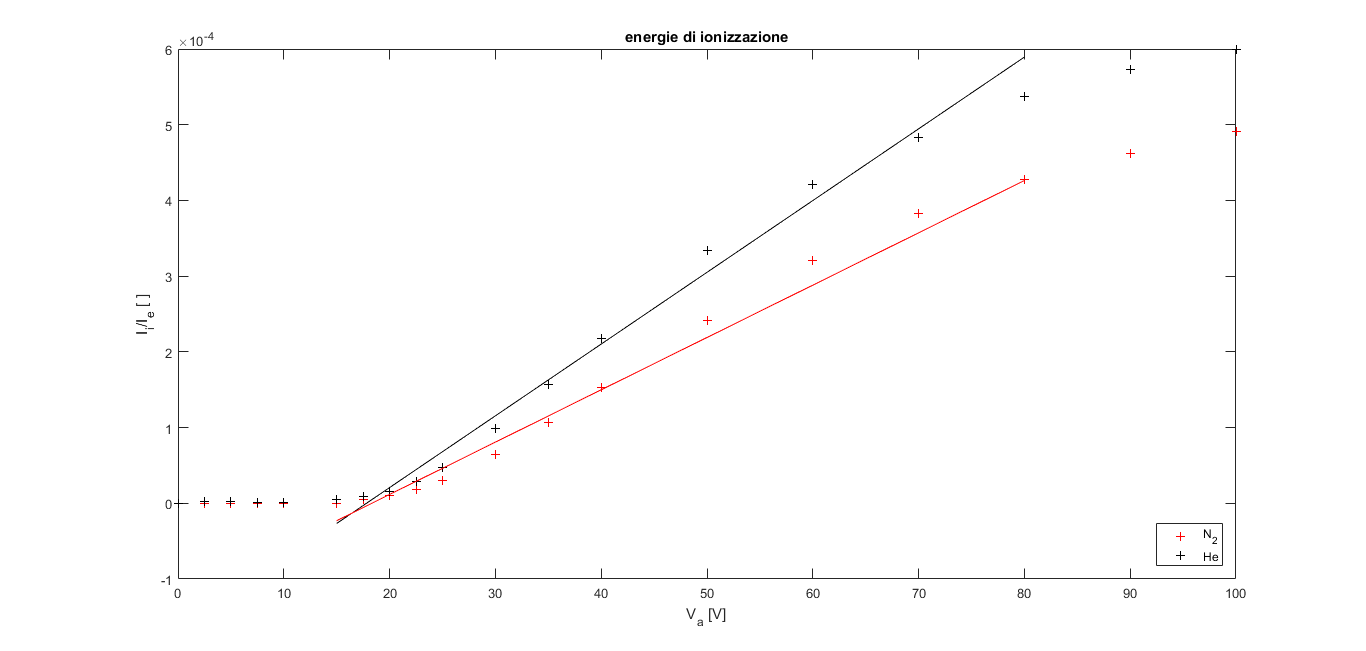
\includegraphics[width=\textwidth]{fig1}
\end{figure}

\end{document}
